\documentclass{beamer}
\usetheme{Madrid}
\usepackage{tikz}
\usepackage{booktabs}
\usetikzlibrary{positioning}
\title{Designing Markets: Chapter 4 Summary}
\subtitle{Handbook of Market Design}
\author{Mohammed Alyahya}
\date{\today}

\begin{document}

% Slide 1: Title
\begin{frame}
    \titlepage
\end{frame}

% Slide 2: What is Market Design?
\begin{frame}{What is Market Design?}
    \begin{itemize}
        \item Market design creates rules and procedures for transactions.
        \item It aims to solve failures in existing or new markets.
        \item Core goals: diagnose failures, evaluate designs, propose improvements.
        \item Success is measured by efficient, fair outcomes.
    \end{itemize}
    \vspace{0.4em}
    \begin{block}{Quick Example}
        Kidney exchange programs match donors and recipients who are incompatible within pairs.
    \end{block}
\end{frame}

% Slide 3: The Three Pillars
\begin{frame}{Three Pillars of Market Design}
    \begin{itemize}
        \item Thickness: Many participants at once.
        \item Safety: Truthful participation is encouraged.
        \item Congestion: Transactions are processed efficiently.
    \end{itemize}
    \vspace{0.6em}
    \centering
    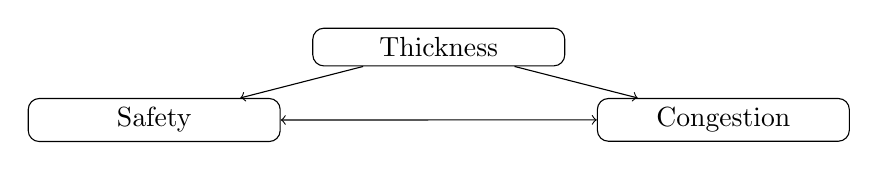
\begin{tikzpicture}[node distance=1.2cm, every node/.style={draw, rounded corners, align=center, minimum width=3.2cm}]
        \node (t) {Thickness};
        \node (s) [below left=0.4cm and 0.4cm of t] {Safety};
        \node (c) [below right=0.4cm and 0.4cm of t] {Congestion};
        \draw[->] (t) -- (s);
        \draw[->] (t) -- (c);
        \draw[<->] (s) -- (c);
    \end{tikzpicture}
\end{frame}

% Slide 4: Diagnosing Market Failures
\begin{frame}{Diagnosing Market Failures}
    \begin{itemize}
        \item Failures often result from poor timing or rules.
        \item Congestion and lack of thickness are common issues.
        \item Example: Residency match programs before redesign.
    \end{itemize}
    \vspace{0.4em}
    \begin{block}{Symptoms}
        Early contracting, thin participation, and strategic misreporting.
    \end{block}
    \vspace{0.2em}
    \centering
    \begin{tabular}{@{}ll@{}}
        \toprule
        Symptom & Likely Cause \\
        \midrule
        Early offers & Timing pressure \\
        Low participation & Thin market \\
        Strategic ranking & Unsafe rules \\
        \bottomrule
    \end{tabular}
\end{frame}

% Slide 5: Real-World Applications
\begin{frame}{Real-World Applications}
    \begin{itemize}
        \item Medical residency matches (NRMP)
        \item Public school choice systems
        \item Kidney exchanges
    \end{itemize}
    \vspace{0.6em}
    \centering
    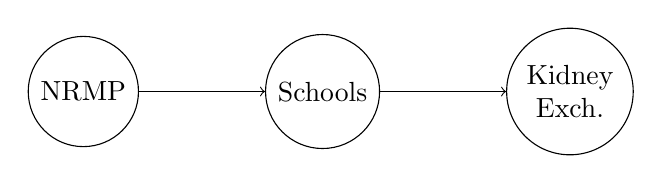
\begin{tikzpicture}[every node/.style={draw, circle, minimum size=1.2cm, align=center}]
        \node (a) {NRMP};
        \node (b) [right=1.6cm of a] {Schools};
        \node (c) [right=1.6cm of b] {Kidney\\Exch.};
        \draw[->] (a) -- (b);
        \draw[->] (b) -- (c);
    \end{tikzpicture}
\end{frame}

% Slide 6: Evaluating and Comparing Designs
\begin{frame}{Evaluating and Comparing Designs}
    \vspace{0.2em}
    \textbf{Central purpose:} compare mechanisms counterfactually across multiple, often competing, dimensions.
    \vspace{0.4em}
    \scriptsize
    \setlength{\extrarowheight}{0pt}
    \begin{tabular}{@{}p{3.6cm}p{6.8cm}@{}}
        \toprule
        Criterion & Description \\
        \midrule
        Allocative efficiency & How well the mechanism realizes mutually beneficial trades; measured by total surplus or match rates. \\\[0.08em]
        Incentive properties & Strategy-proofness, robustness to manipulation, and the reliance on equilibrium play. \\\[0.08em]
        Distributional outcomes & How surplus or access is distributed; which groups are advantaged or disadvantaged. \\\[0.08em]
        Fairness & Absence of justified envy, respect for priority rights, and transparent procedures. \\\[0.08em]
        Participation & Take-up rates, accessibility, and whether complexity deters honest participation. \\\[0.08em]
        Practical robustness & Administrat‹ive feasibility, legal constraints, and sensitivity to shocks. \\
        \bottomrule
    \end{tabular}
    \vspace{0.35em}
    \begin{block}{Example}
        Deferred Acceptance vs First-come-first-served: DA raises stability and centralized participation (reducing unraveling and strategic premia), while FCFS can be faster but increases incentives for early contracting and inequitable outcomes.
    \end{block}
\end{frame}

% Slide 7: Mechanism Stability
\begin{frame}{Mechanism Stability}
    \begin{itemize}
        \item A matching is stable if no pair prefers each other over current matches.
        \item Stability is crucial for long-term market health.
    \end{itemize}
    \vspace{0.4em}
    \begin{block}{Why it matters}
        Instability encourages participants to bypass the mechanism.
    \end{block}
\end{frame}

% Slide 8: Participation and Thickness
\begin{frame}{Participation and Thickness}
    \begin{itemize}
        \item Participation incentives can be more important than optimal rules.
        \item Thin markets reduce matching quality and raise strategic behavior.
        \item Centralization and timing coordination help build thickness.
    \end{itemize}
    \vspace{0.4em}
    \begin{block}{Example}
        Kidney exchange platforms improve outcomes when hospitals contribute more pairs.
    \end{block}
\end{frame}

% Slide 9: Redesign Principles
\begin{frame}{Redesign Principles}
    \begin{itemize}
        \item Start with diagnosis, then test alternatives with data or simulations.
        \item Preserve incentives: stability, transparency, and simplicity matter.
        \item Iterate: small rule changes can shift outcomes significantly.
    \end{itemize}
    \vspace{0.4em}
    \begin{block}{Rule of Thumb}
        Design for participation first, then refine for efficiency and fairness.
    \end{block}
\end{frame}

% Slide 10: Conclusion
\begin{frame}{Conclusion}
    \begin{itemize}
        \item Effective market design requires diagnosis and iteration.
        \item AI tools help simulate and verify market rules.
        \item Design cycle: diagnose $\rightarrow$ evaluate $\rightarrow$ redesign.
    \end{itemize}
    \vspace{0.4em}
    \begin{block}{Takeaway}
        Good design aligns incentives, improves participation, and reduces congestion.
    \end{block}
\end{frame}

\end{document}
